\documentclass[11pt]{article}
\usepackage[margin=2.4cm]{geometry}
\usepackage[T1]{fontenc}
\usepackage{graphicx}
\usepackage{booktabs}
\usepackage{threeparttable}
\usepackage{lineno}
\usepackage{caption}
\usepackage{placeins}
\usepackage[hidelinks]{hyperref}
\captionsetup{font=small,labelfont=bf}
\newcommand{\auc}{\ensuremath{\mathrm{ROC\mbox{-}AUC}}}
\title{Motor-imagery EEG decoding under simulated channel loss and reduced montages}
\author{Anna Nikolaevna Sokolova\\
\small Southern Federal University, Rostov-on-Don, Russia\\
\small ORCID: \href{https://orcid.org/0009-0000-5733-9994}{0009-0000-5733-9994}\\
\small Correspondence: \href{mailto:ansokolova@sfedu.ru}{ansokolova@sfedu.ru}}
\date{}

\begin{document}
\maketitle
\linenumbers

\begin{abstract}
\textbf{Background:} Motor-imagery electroencephalography (EEG) decoders are commonly evaluated on clean recordings. We evaluated how two offline decoders behave under controlled channel zeroing and when retrained on reduced montages, with inference at the participant level.

\textbf{Methods:} Common spatial patterns with linear discriminant analysis (CSP--LDA) and covariance-based Riemannian tangent-space logistic regression (Riemann--LR) were evaluated on PhysioNet Motor Movement/Imagery data (109 participants) and BNCI2014-001 (9 participants). The primary outcome was receiver operating characteristic area under the curve (ROC-AUC). Stressors comprised random test-time channel dropout (10--50\%), three predefined motor-region dropouts, 3- and 9-channel montages, and cross-session transfer when usable session metadata were available. Fold and repeat measurements were collapsed within participant. Paired tests, 95\% confidence intervals, Cohen's $d_z$, Wilcoxon sensitivity tests, and Benjamini--Hochberg correction were used.

\textbf{Results:} On PhysioNet, 50\% random dropout reduced mean ROC-AUC from 0.655 to 0.527 for CSP--LDA (mean paired change $-0.128$, 95\% CI $-0.153$ to $-0.102$) and from 0.675 to 0.554 for Riemann--LR ($-0.121$, 95\% CI $-0.141$ to $-0.101$). Riemann--LR had higher absolute ROC-AUC at all four random-dropout levels. In an exploratory paired difference-in-degradation analysis, its loss from clean was smaller at 10--30\% dropout, but not detectably smaller at 50\% dropout. For the 9-channel montage, mean changes from the full montage were 0.014 for CSP--LDA and 0.001 for Riemann--LR; the confidence intervals included both small losses and small gains, and equivalence was not tested. Cross-session evidence was available only in BNCI2014-001 and was imprecise because $n=9$.

\textbf{Conclusions:} Test-time channel zeroing reduced participant-level ROC-AUC for both pipelines. Riemann--LR had higher absolute ROC-AUC in the tested random- and regional-dropout conditions. Estimates for the 9-channel montage were close to the full-montage estimates, but equivalence was not established. These findings apply to offline binary motor-imagery decoding and the corruption models evaluated here.
\end{abstract}

\noindent\textbf{Keywords:} brain--computer interface; electroencephalography; motor imagery; robustness; channel dropout; common spatial patterns; Riemannian geometry; reproducibility

\section{Introduction}
Motor-imagery brain--computer interfaces (BCIs) translate electroencephalographic activity into control signals without requiring overt movement. Their relevance to assistive control depends on performance outside a clean, fixed laboratory setup. Electrode impedance changes, disconnected leads, cap displacement, and reduced wearable montages can alter the spatial information presented to a decoder. A model that performs well on intact recordings may therefore fail when deployed.

Public datasets and benchmarking software have improved reproducibility in BCI research. PhysioNet provides openly accessible physiological recordings and associated software infrastructure \cite{Goldberger_2000}; its EEG Motor Movement/Imagery corpus was acquired using BCI2000 \cite{Schalk_2004} and has recently been curated to improve accessibility for decoding studies \cite{Shuqfa_2024}. BNCI2014-001 is widely used as data set 2a of BCI Competition IV \cite{Tangermann_2012}. The Mother of All BCI Benchmarks (MOABB) supports standardized access and evaluation across such datasets \cite{Jayaram_2018}. These resources reduce dataset and implementation variability, but standard accuracy estimates do not directly quantify behavior under predefined test-time channel perturbations.

We examined two established decoder families. Common spatial patterns (CSP) construct spatial filters that discriminate motor-imagery classes \cite{Ramoser_2000}. Riemannian approaches represent trial covariance matrices on the manifold of symmetric positive-definite matrices and have been effective for BCI classification \cite{Barachant_2012}. Their different representations suggest different responses to missing channels, but a comparison must pair models within the same participants and perturbation conditions.

This study had three objectives: (1) quantify within-participant degradation caused by random and spatially clustered test-time channel loss; (2) estimate changes after retraining on reduced motor-centered montages; and (3) compare CSP--LDA with Riemann--LR under matched PhysioNet conditions. The contribution is an explicit perturbation protocol rather than a new classifier. Fold and repeat measurements are retained, while population inference is performed after participant-level aggregation.

\section{Materials and methods}
\subsection{Datasets and analysis cohorts}
We used two open motor-imagery EEG datasets through MOABB. PhysioNet Motor Movement/Imagery contributed 109 participants to each full decoder analysis. BNCI2014-001 contributed all 9 participants. The task was binary left-versus-right motor imagery, implemented through the MOABB \texttt{LeftRightImagery} paradigm. EEG was band-pass filtered from 8 to 32~Hz and resampled to 128~Hz by the paradigm interface. Raw EEG files were not redistributed.

The PhysioNet fold-level files contained 25,070 rows per decoder and yielded 1,090 participant-condition rows per decoder. Both PhysioNet cohorts contained all 109 participants, and fold-to-participant aggregation passed the prespecified validation checks. BNCI analyses contained 90 participant-condition rows per decoder.

\subsection{Decoder pipelines}
The CSP--LDA pipeline used six CSP components, logarithmic component power, no trace normalization, and linear discriminant analysis. For a three-channel montage, the component count was limited to the number of available channels. The Riemann--LR pipeline estimated trial covariance matrices using Oracle Approximating Shrinkage, mapped them to the Riemannian tangent space, and fitted logistic regression with a maximum of 2,000 iterations. The same random seed (42) was used throughout. The reported analyses used six CSP components and Oracle Approximating Shrinkage; neither was selected using test-fold performance. The 8--32~Hz band was chosen to cover the conventional mu and beta ranges used in motor-imagery decoding; alternative bands and component counts were not evaluated in this study.

\subsection{Cross-validation and perturbations}
Within each participant, intact-data performance and test-time perturbations were evaluated with shuffled stratified five-fold cross-validation. The effective fold count was reduced only if the smaller class contained fewer than five trials. A decoder was fitted on intact training folds. Random dropout then set the same sampled channel subset to zero across every epoch in the corresponding test fold. Dropout fractions were 0.10, 0.20, 0.30, and 0.50, with 10 repeats per fraction; the clean condition used one evaluation per fold. Random draws were deterministic functions of seed, fold, repeat, and fraction. The four fractions covered mild to severe channel loss. Ten channel masks were evaluated per fraction and fold. The legacy reproduction protocol used for the reported tables did not include participant identity in the mask seed. Consequently, matched fold, repeat, and fraction indices used the same channel indices across participants when channel order was the same. This preserves matching between decoders but does not sample independent mask schedules across participants. Reported intervals are therefore conditional on this schedule; alternative masks, cross-validation splits, and repeat counts were not evaluated. The repository also supplies a corrected prospective configuration with participant-specific masks, but no results from that configuration are reported here.

Spatially clustered dropout set predefined channels to zero only in the test fold. The PhysioNet definitions were left motor strip (FC5, FC3, FC1, C5, C3, C1, CP5, CP3, CP1), midline motor strip (FCz, Cz, CPz), and right motor strip (FC2, FC4, FC6, C2, C4, C6, CP2, CP4, CP6), restricted to channels present in a dataset. These corresponded to 9/64, 3/64, and 9/64 PhysioNet channels.

Reduced-montage analyses differed from dropout analyses: both training and test data were restricted to the same channels. The motor-core montage contained C3, Cz, and C4. The motor-extended montage contained FC3, FCz, FC4, C3, Cz, C4, CP3, CPz, and CP4. Cross-session analysis trained on the first available session and tested on later sessions when metadata exposed at least two usable sessions with both classes. This produced BNCI2014-001 results but no PhysioNet results.

\subsection{Outcomes and statistical analysis}
The primary outcome reported here was ROC-AUC. Balanced accuracy was secondary. Brier score and 10-bin equal-width expected calibration error were calculated when probability estimates were available.

Fold and repeat rows were first averaged within participant and condition. Population inference therefore used participants, not folds or repeats, as independent units. Population-level condition means used subject-level bias-corrected and accelerated bootstrap intervals with 2,000 resamples and seed 42. Each stressor was compared with the participant's clean all-channel result. For paired changes, we report a two-sided 95\% Student $t$ interval, paired $t$ test, Cohen's $d_z$, Wilcoxon signed-rank sensitivity test, and an exact sign test. Benjamini--Hochberg false-discovery-rate correction was applied within each test family across available conditions \cite{Benjamini_1995}. Shapiro--Wilk tests described the distribution of paired changes.

For the direct PhysioNet decoder comparison, subject and condition were matched one-to-one. The primary cross-pipeline estimand was ROC-AUC for CSP--LDA minus ROC-AUC for Riemann--LR; negative values favor Riemann--LR. An exploratory difference-in-degradation estimand subtracted the clean-condition cross-pipeline difference from each non-clean cross-pipeline difference. It therefore compares within-subject changes from each decoder's own clean baseline. We report the proportion of participants for whom CSP--LDA was better and exact binomial confidence intervals. The three regional-dropout conditions were matched directly by anatomical region name. No regional rows were averaged and no missing observations were imputed.

Two maximum-likelihood mixed-effects models with participant random intercepts were used as secondary analyses: a categorical condition model referenced to clean data, and a continuous dropout-fraction model restricted to clean plus random-dropout rows. We assessed convergence, near-zero random-intercept variance, residual normality with the Shapiro--Wilk test, heteroscedasticity with the Breusch--Pagan test, quadratic dose response, functional form with Ramsey RESET, and leave-one-participant-out coefficient influence. Mixed-model estimates were not treated as the sole inferential evidence when diagnostics failed.

\subsection{Software, validation, and reproducibility}
The benchmark was implemented in Python using MNE, MOABB, scikit-learn, pyRiemann, SciPy, pandas, and statsmodels. A pinned CPython 3.11/Linux environment is provided in \texttt{requirements-lock.txt}. Repository checks cover schemas, metric ranges, duplicate keys, channel counts, clean-baseline pairing, expected participant counts, and agreement between fold- and participant-level summaries. Raw EEG caches and temporary checkpoints are not included in the repository.

\begin{figure}[t]
\centering
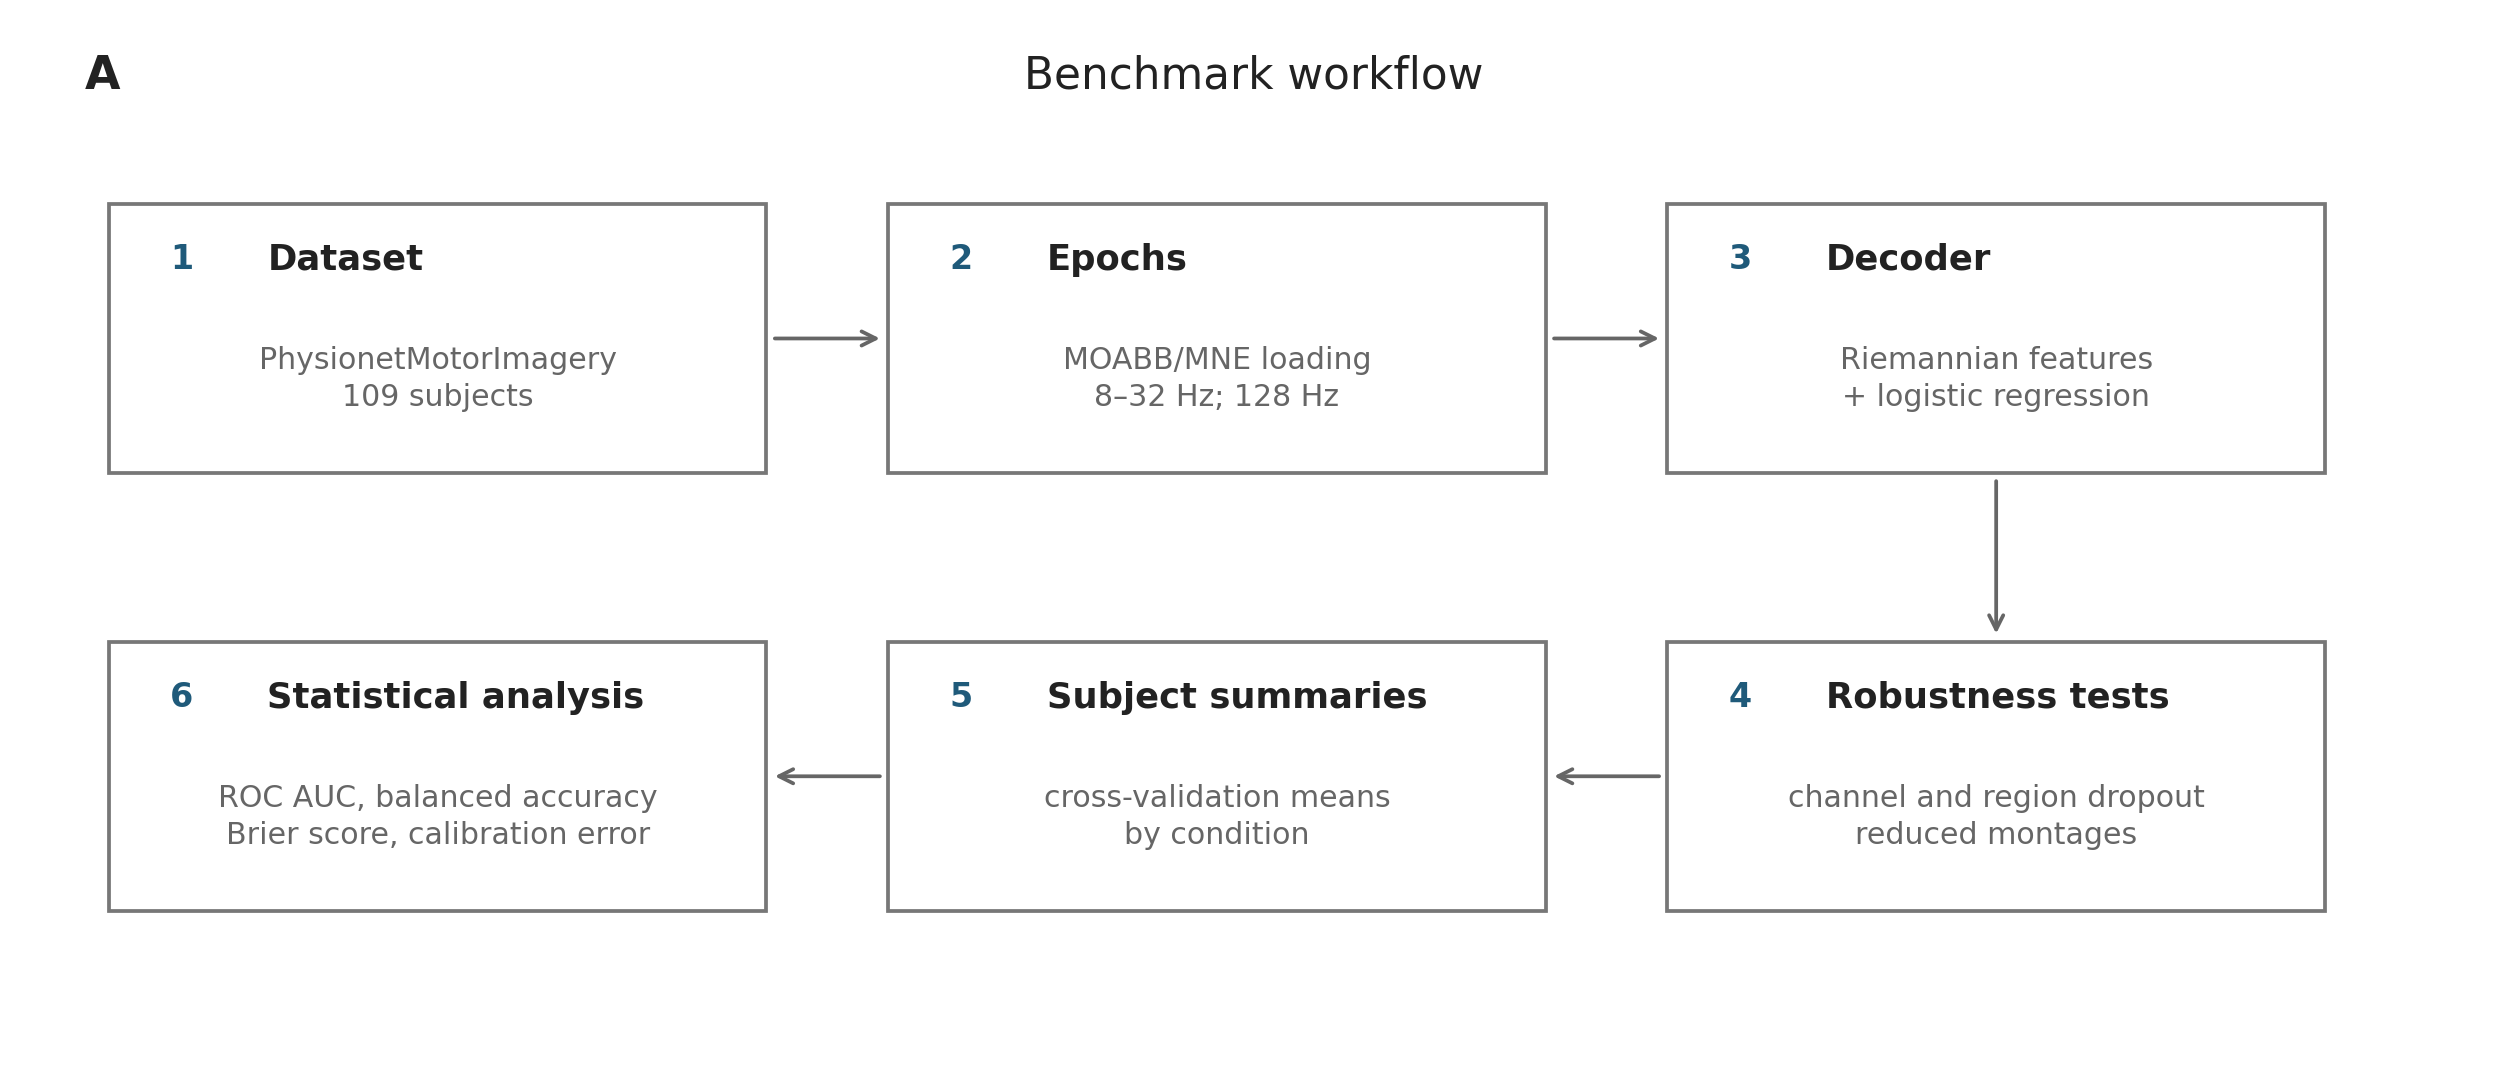
\includegraphics[width=0.98\linewidth]{figure1_benchmark_pipeline.png}
\caption{Benchmark workflow. EEG was loaded through MOABB, evaluated with CSP--LDA or Riemann--LR, exposed to clean, dropout, montage, and available cross-session conditions, and collapsed to participant-level summaries before inference. The diagram is generated by the repository reporting code.}
\label{fig:pipeline}
\end{figure}

\section{Results}
\subsection{PhysioNet performance under random channel dropout}
Both decoders degraded as random test-time channel loss increased (Table~\ref{tab:main}). For CSP--LDA, mean ROC-AUC decreased from 0.655 on clean data to 0.527 at 50\% dropout. The paired change was $-0.128$ (95\% CI $-0.153$ to $-0.102$; $d_z=-0.944$; false-discovery-rate-adjusted paired $t$-test $p=2.55\times10^{-16}$; adjusted Wilcoxon $p=4.94\times10^{-13}$). For Riemann--LR, mean ROC-AUC decreased from 0.675 to 0.554. The paired change was $-0.121$ (95\% CI $-0.141$ to $-0.101$; $d_z=-1.135$; adjusted paired $t$-test $p=8.12\times10^{-21}$; adjusted Wilcoxon $p=4.83\times10^{-15}$).

\begin{table}[t]
\centering
\caption{Primary PhysioNet results at 50\% random channel dropout and reduced montages. Changes compare each condition with the same participant's clean all-channel result.}
\label{tab:main}
\begin{threeparttable}
\small
\begin{tabular}{llrrrr}
\toprule
Decoder & Condition & Mean AUC & Paired change & 95\% CI & $d_z$ \\
\midrule
CSP--LDA & Clean & 0.655 & --- & --- & --- \\
CSP--LDA & 50\% dropout & 0.527 & $-0.128$ & [$-0.153$, $-0.102$] & $-0.944$ \\
CSP--LDA & Motor core & 0.648 & $-0.007$ & [$-0.035$, 0.021] & $-0.046$ \\
CSP--LDA & Motor extended & 0.669 & 0.014 & [$-0.013$, 0.040] & 0.097 \\
\addlinespace
Riemann--LR & Clean & 0.675 & --- & --- & --- \\
Riemann--LR & 50\% dropout & 0.554 & $-0.121$ & [$-0.141$, $-0.101$] & $-1.135$ \\
Riemann--LR & Motor core & 0.639 & $-0.036$ & [$-0.064$, $-0.009$] & $-0.248$ \\
Riemann--LR & Motor extended & 0.677 & 0.001 & [$-0.027$, 0.030] & 0.010 \\
\bottomrule
\end{tabular}
\begin{tablenotes}\footnotesize
\item $n=109$ for every row. AUC, receiver operating characteristic area under the curve; CI, confidence interval; $d_z$, standardized mean paired change.
\end{tablenotes}
\end{threeparttable}
\end{table}

\subsection{Direct comparison of decoders}
Riemann--LR had higher absolute mean ROC-AUC at all four random-dropout fractions (Figure~\ref{fig:comparison}; Table~\ref{tab:comparison}). The mean paired difference was $-0.050$ at 10\% dropout, $-0.051$ at 20\%, $-0.051$ at 30\%, and $-0.027$ at 50\%. All four confidence intervals excluded zero. Adjusted paired $t$-test $p$ values ranged from $1.02\times10^{-4}$ to 0.014; adjusted Wilcoxon $p$ values ranged from $1.71\times10^{-4}$ to 0.028. Riemann--LR was better for 61--71 of 109 participants across these conditions.

The exploratory difference-in-degradation analysis separated the clean-condition gap from the response to dropout (Table~\ref{tab:degradation-contrast}). The mean contrast, defined as change in CSP--LDA minus change in Riemann--LR, was $-0.029$ at 10\% dropout (95\% CI $-0.045$ to $-0.014$), $-0.030$ at 20\% ($-0.050$ to $-0.010$), $-0.031$ at 30\% ($-0.051$ to $-0.011$), and $-0.007$ at 50\% ($-0.028$ to 0.014). Benjamini--Hochberg-adjusted paired $t$-test $p$ values were 0.001, 0.007, 0.007, and 0.533, respectively. Thus, the data supported a smaller Riemann--LR loss at 10--30\% dropout, but not at 50\% dropout.

\begin{table}[t]
\centering
\caption{Exploratory paired difference in degradation from each decoder's clean baseline. Negative contrasts indicate a larger CSP--LDA loss.}
\label{tab:degradation-contrast}
\begin{threeparttable}
\small
\begin{tabular}{lrrrr}
\toprule
Dropout & CSP change & Riemann change & Contrast [95\% CI] & Adjusted $p$ \\
\midrule
10\% & $-0.065$ & $-0.036$ & $-0.029$ [$-0.045$, $-0.014$] & 0.001 \\
20\% & $-0.102$ & $-0.071$ & $-0.030$ [$-0.050$, $-0.010$] & 0.007 \\
30\% & $-0.112$ & $-0.081$ & $-0.031$ [$-0.051$, $-0.011$] & 0.007 \\
50\% & $-0.128$ & $-0.121$ & $-0.007$ [$-0.028$, 0.014] & 0.533 \\
\bottomrule
\end{tabular}
\begin{tablenotes}\footnotesize
\item $n=109$ for every row. Adjusted $p$ values use the Benjamini--Hochberg procedure across nine non-clean conditions; the table displays the four random-dropout contrasts.
\end{tablenotes}
\end{threeparttable}
\end{table}

The clean-data difference was $-0.020$ (95\% CI $-0.042$ to 0.001). The adjusted paired $t$ test did not reject equality ($p=0.079$), whereas the adjusted Wilcoxon test did ($p=0.049$). We therefore do not claim a clean-condition difference supported by both tests. Neither reduced montage showed a clear between-decoder difference: motor core 0.009 (95\% CI $-0.002$ to 0.020) and motor extended $-0.008$ (95\% CI $-0.021$ to 0.004).

For regional dropout, Riemann--LR exceeded CSP--LDA in each anatomically matched comparison. Differences were $-0.039$ for the left motor strip (95\% CI $-0.064$ to $-0.014$; $d_z=-0.296$), $-0.056$ for the midline motor strip (95\% CI $-0.082$ to $-0.030$; $d_z=-0.411$), and $-0.034$ for the right motor strip (95\% CI $-0.059$ to $-0.009$; $d_z=-0.260$).

\begin{figure}[t]
\centering
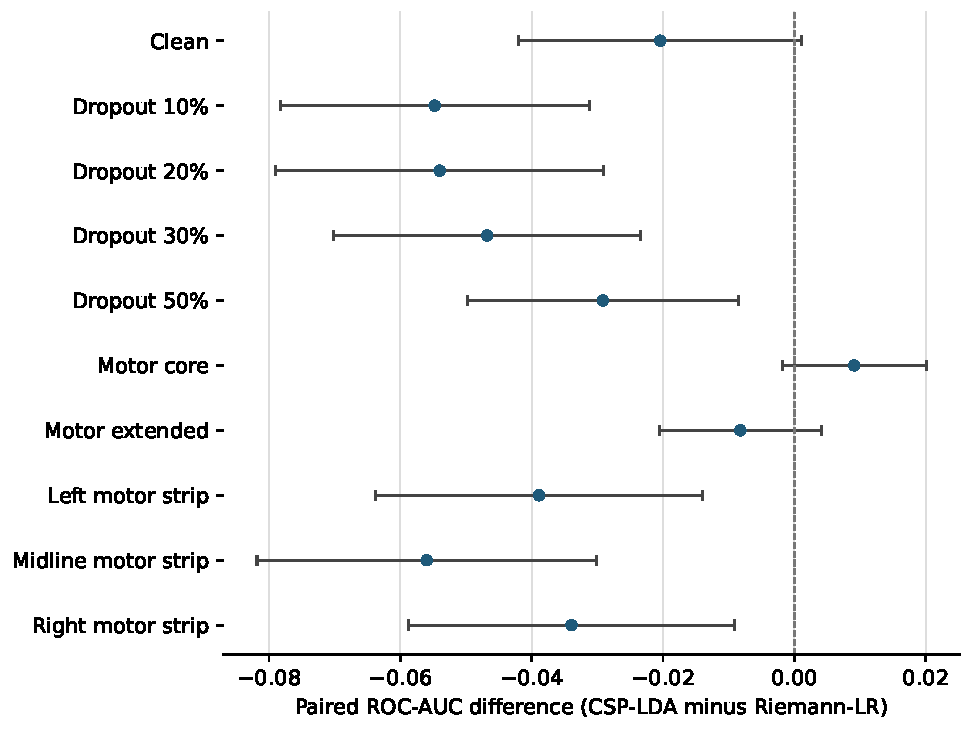
\includegraphics[width=0.92\linewidth]{figure2_paired_decoder_comparison.pdf}
\caption{Subject-paired PhysioNet decoder comparison. Points are mean differences in ROC-AUC (CSP--LDA minus Riemann--LR); bars are 95\% Student $t$ confidence intervals; $n=109$ for every condition. Negative values favor Riemann--LR. The three regional comparisons are matched directly by anatomical region name.}
\label{fig:comparison}
\end{figure}

\begin{table}[t]
\centering
\caption{Matched PhysioNet comparison of CSP--LDA and Riemann--LR.}
\label{tab:comparison}
\begin{threeparttable}
\scriptsize
\begin{tabular}{lrrrrr}
\toprule
Condition & CSP mean & Riemann mean & Difference [95\% CI] & $d_z$ & CSP better \\
\midrule
Clean & 0.655 & 0.675 & $-0.020$ [$-0.042$, 0.001] & $-0.180$ & 39/109 \\
Dropout 10\% & 0.590 & 0.640 & $-0.050$ [$-0.072$, $-0.028$] & $-0.427$ & 38/109 \\
Dropout 20\% & 0.553 & 0.604 & $-0.051$ [$-0.075$, $-0.027$] & $-0.399$ & 42/109 \\
Dropout 30\% & 0.543 & 0.594 & $-0.051$ [$-0.074$, $-0.028$] & $-0.427$ & 39/109 \\
Dropout 50\% & 0.527 & 0.554 & $-0.027$ [$-0.048$, $-0.007$] & $-0.251$ & 48/109 \\
Motor core & 0.648 & 0.639 & 0.009 [$-0.002$, 0.020] & 0.159 & 54/109 \\
Motor extended & 0.669 & 0.677 & $-0.008$ [$-0.021$, 0.004] & $-0.127$ & 53/109 \\
Left motor strip & 0.597 & 0.636 & $-0.039$ [$-0.064$, $-0.014$] & $-0.296$ & 38/109 \\
Midline motor strip & 0.607 & 0.663 & $-0.056$ [$-0.082$, $-0.030$] & $-0.411$ & 35/109 \\
Right motor strip & 0.594 & 0.628 & $-0.034$ [$-0.059$, $-0.009$] & $-0.260$ & 39/109 \\
\bottomrule
\end{tabular}
\begin{tablenotes}\footnotesize
\item Difference is CSP--LDA minus Riemann--LR. ``CSP better'' counts strict positive differences; ties are excluded from this count but retained in the denominator shown.
\end{tablenotes}
\end{threeparttable}
\end{table}

\subsection{Reduced montages}
For the 9-channel motor-extended montage, CSP--LDA changed by 0.014 (95\% CI $-0.013$ to 0.040; adjusted paired $t$-test $p=0.333$), and Riemann--LR changed by 0.001 (95\% CI $-0.027$ to 0.030; $p=0.947$). These intervals were compatible with both a small loss and a small gain. No equivalence or non-inferiority margin was specified. The 3-channel motor-core montage also showed no clear CSP--LDA change ($-0.007$, 95\% CI $-0.035$ to 0.021; $p=0.635$), but Riemann--LR decreased by $-0.036$ (95\% CI $-0.064$ to $-0.009$; $p=0.012$).

\subsection{BNCI2014-001 sensitivity analysis and cross-session transfer}
The smaller BNCI2014-001 cohort showed larger losses at 50\% random dropout. CSP--LDA decreased from 0.852 to 0.616 (paired change $-0.236$, 95\% CI $-0.293$ to $-0.179$; $n=9$), and Riemann--LR decreased from 0.878 to 0.721 ($-0.157$, 95\% CI $-0.200$ to $-0.113$). Cross-session estimates did not show clear ROC-AUC changes: 0.001 for CSP--LDA (95\% CI $-0.021$ to 0.023) and $-0.007$ for Riemann--LR (95\% CI $-0.022$ to 0.007). The cohort is too small for strong population claims, and cross-session results were unavailable in the larger PhysioNet cohort.

\subsection{Model diagnostics}
Both mixed-effects models converged, and leave-one-participant-out influence checks did not identify a coefficient change above the implemented relative threshold. Residual diagnostics rejected normality and constant variance for both decoder families. The subject-demeaned quadratic and Ramsey RESET tests also rejected a strictly linear random-dropout dose response. The continuous mixed-model slope is therefore a descriptive summary across tested fractions rather than evidence that degradation is linear. Participant-paired estimates and Wilcoxon sensitivity analyses are the main inferential results.

\section{Discussion}
This benchmark produced three findings relevant to evaluation of motor-imagery decoders. First, large test-time channel loss substantially reduced discrimination for both pipelines. At 50\% dropout, mean PhysioNet ROC-AUC fell by about 0.12 for each decoder. Second, Riemann--LR had higher absolute ROC-AUC than CSP--LDA under every tested level of random dropout and under all three anatomically matched regional-dropout comparisons. The standardized between-decoder effects were small to moderate ($|d_z|=0.25$--$0.43$), so the result concerns relative robustness rather than immunity to channel loss. Third, estimates for the 9-channel motor-centered montage were close to the full-montage estimates, but equivalence was not tested; planned sensor reduction and unplanned channel zeroing are different estimands.

The distinction between dropout and reduced montage is methodological. Dropout models a decoder trained on intact spatial information and then evaluated after sensor loss. Zeroed channels do not recreate every physical failure mode, but they provide a controlled test of missing signal input. Reduced-montage models are retrained on the smaller channel set, allowing their spatial representation to adapt. The 9-channel estimates therefore do not imply that nine arbitrary failed channels are harmless. They motivate a prespecified non-inferiority study of retraining for a stable, motor-centered layout.

Part of Riemann--LR's absolute advantage under dropout was already present in the clean condition. The exploratory difference-in-degradation analysis supported a smaller loss at 10--30\% dropout, but not at 50\% dropout. A covariance representation retaining useful distributed structure is one possible interpretation, not a mechanism established here. The clean-condition evidence was mixed between the paired $t$ and Wilcoxon tests, and reduced-montage differences were not clear. Decoder selection should therefore consider the intended failure model instead of relying on one intact-data ranking.

The analysis addresses common statistical weaknesses in repeated benchmark outputs. Folds and dropout repeats are not treated as independent participants. Inference is performed after aggregation to one row per participant and condition. Parametric estimates are accompanied by signed-rank sensitivity tests and false-discovery-rate correction. Diagnostics show why this matters: residual normality, homoscedasticity, and linear dose-response assumptions did not hold. Reporting only the linear mixed-model slope would overstate the adequacy of that functional form.

\subsection{Limitations}
Several limitations restrict interpretation. PhysioNet did not yield usable cross-session rows, leaving only nine BNCI participants for that analysis. Zero-valued channels approximate complete signal loss but do not model impedance noise, bridging, clipping, intermittent contact, or online recalibration. The random-dropout estimates are conditional on one shuffled cross-validation split and one deterministic mask schedule shared across participants at matched fold and repeat indices; split and mask-schedule sensitivity were not measured. Within-participant cross-validation pooled available sessions and runs rather than enforcing leave-session or leave-run separation, except in the separate BNCI cross-session analysis. The analysis was not preregistered, so the distinction between confirmatory and exploratory results rests on the reporting plan in this repository rather than a time-stamped protocol. Results from two classical pipelines and two public datasets do not cover deep networks, regression control, asynchronous operation, or users with motor impairment. Finally, offline discrimination cannot establish clinical benefit, online controllability, safety, or a causal treatment effect.

Future work should preserve fold-level and anatomical-condition provenance for every pipeline, add prospective corruption models beyond zeroing, and evaluate recalibration strategies under independently generated, documented stressor schedules. Larger multi-session cohorts are needed for cross-session inference. Extension to continuous control should use outcomes linked to command latency, trajectory error, and task completion rather than classification metrics alone.

\section{Conclusions}
In these offline analyses, channel zeroing reduced ROC-AUC for both decoders. Riemann--LR had higher absolute ROC-AUC than CSP--LDA in the tested PhysioNet dropout conditions, but both pipelines approached weak discrimination at 50\% dropout. The reduced-montage results do not establish equivalence. A full rerun with independent cross-validation splits and the supplied participant-specific mask schedule is required before treating the observed decoder differences as stable.

\section*{Data and code availability}
The analysis uses public datasets accessed through MOABB and MNE; raw EEG is not redistributed. The manuscript is linked to software release version 0.3.1. The repository (\url{https://github.com/ZyntZ/BCI-Prosthesis-Robustness-Benchmark}) contains the benchmark code, pinned dependencies, fold-level and participant-level results, statistical tables, and validation output. A permanent repository DOI has not yet been assigned and should be added to the accepted manuscript and software citation after archival release.

\section*{Ethics statement}
This study performed a secondary analysis of two publicly accessible, de-identified datasets and recruited no new participants. The author did not interact with participants, access direct identifiers, or redistribute raw EEG. The PhysioNet EEG Motor Movement/Imagery repository identifies the data as open access under the Open Data Commons Attribution License v1.0, and the BNCI Horizon 2020 repository distributes BNCI2014-001 under the Creative Commons Attribution-NoDerivatives 4.0 International License. The repository pages and the BNCI2014-001 dataset description consulted for this analysis do not report ethics-committee names, approval identifiers, or consent wording for the original acquisitions. Therefore, no such details are asserted here. Confirmation from the original data custodians may be required if the journal requests acquisition-level approval or consent documentation. No new ethics-approval identifier is reported for this secondary analysis; an institutional exemption or not-required determination should be supplied if requested by the journal or required by the author's institution.

\section*{Funding}
This research did not receive any specific grant from funding agencies in the public, commercial, or not-for-profit sectors.

\section*{CRediT authorship contribution statement}
Anna Nikolaevna Sokolova: Conceptualization, Methodology, Software, Validation, Formal analysis, Investigation, Data curation, Visualization, Writing -- original draft, Writing -- review and editing, Project administration.

\FloatBarrier
\begin{thebibliography}{99}
\bibitem{Goldberger_2000} Goldberger AL, Amaral LAN, Glass L, et al. PhysioBank, PhysioToolkit, and PhysioNet: components of a new research resource for complex physiologic signals. \textit{Circulation}. 2000;101:e215--e220. \href{https://doi.org/10.1161/01.CIR.101.23.e215}{doi:10.1161/01.CIR.101.23.e215}.
\bibitem{Schalk_2004} Schalk G, McFarland DJ, Hinterberger T, Birbaumer N, Wolpaw JR. BCI2000: a general-purpose brain--computer interface system. \textit{IEEE Trans Biomed Eng}. 2004;51:1034--1043. \href{https://doi.org/10.1109/TBME.2004.827072}{doi:10.1109/TBME.2004.827072}.
\bibitem{Shuqfa_2024} Shuqfa Z, Lakas A, Belkacem AN. Increasing accessibility to a large brain--computer interface dataset: curation of PhysioNet EEG Motor Movement/Imagery dataset for decoding and classification. \textit{Data Brief}. 2024;53:110181. \href{https://doi.org/10.1016/j.dib.2024.110181}{doi:10.1016/j.dib.2024.110181}.
\bibitem{Tangermann_2012} Tangermann M, M\"uller KR, Aertsen A, et al. Review of the BCI Competition IV. \textit{Front Neurosci}. 2012;6:55. \href{https://doi.org/10.3389/fnins.2012.00055}{doi:10.3389/fnins.2012.00055}.
\bibitem{Jayaram_2018} Jayaram V, Barachant A. MOABB: trustworthy algorithm benchmarking for BCIs. \textit{J Neural Eng}. 2018;15:066011. \href{https://doi.org/10.1088/1741-2552/aadea0}{doi:10.1088/1741-2552/aadea0}.
\bibitem{Ramoser_2000} Ramoser H, Muller-Gerking J, Pfurtscheller G. Optimal spatial filtering of single trial EEG during imagined hand movement. \textit{IEEE Trans Rehabil Eng}. 2000;8:441--446. \href{https://doi.org/10.1109/86.895946}{doi:10.1109/86.895946}.
\bibitem{Barachant_2012} Barachant A, Bonnet S, Congedo M, Jutten C. Multiclass brain--computer interface classification by Riemannian geometry. \textit{IEEE Trans Biomed Eng}. 2012;59:920--928. \href{https://doi.org/10.1109/TBME.2011.2172210}{doi:10.1109/TBME.2011.2172210}.
\bibitem{Benjamini_1995} Benjamini Y, Hochberg Y. Controlling the false discovery rate: a practical and powerful approach to multiple testing. \textit{J R Stat Soc Series B}. 1995;57:289--300. \href{https://doi.org/10.1111/j.2517-6161.1995.tb02031.x}{doi:10.1111/j.2517-6161.1995.tb02031.x}.
\end{thebibliography}
\end{document}
